\documentclass[letterpaper, reqno,11pt]{article}
\usepackage[margin=1.0in]{geometry}
\usepackage{color,latexsym,amsmath,amssymb, listings, graphicx}

\usepackage{hyperref}

\hypersetup{
colorlinks=true,
linkcolor=magenta,
filecolor=magenta,
urlcolor=cyan,
}

\graphicspath{ {images/} }

\newcommand{\RR}{\mathbb{R}}
\newcommand{\CC}{\mathbb{C}}
\newcommand{\ZZ}{\mathbb{Z}}
\newcommand{\QQ}{\mathbb{Q}}
\newcommand{\NN}{\mathbb{N}}
\newcommand{\st}{\mathrm{ s.t.}\ }

\begin{document}
\pagenumbering{arabic}
\title{Elec 221 Homework 1}
\date{September 21, 2021}
\author{Xander Naumenko}
\newtheorem{thm}{Theorem}
\maketitle

\noindent {\bf 1a1.} This is false. First note that the time shift can be related to the phase shift by equating the expression inside the cosine. 

$$
    2\pi f_0 t+\phi=2\pi f_0(t-t_1)) + 2n\pi, n\in\ZZ
$$
$$
    \phi=2\pi f_0 t_1 + 2n\pi, n\in\ZZ
$$
$$
    \phi=-\frac14\pi t_1+2n\pi, n\in\ZZ
$$

Applying this with $t=-2$, we find that the phase shift using this formula is not $\phi=\frac{3\pi}4$

\noindent {\bf 1a2.} This is false. Using the same formula as in part 1 we get $\phi=-\frac14\pi t_1+2n\pi=-\frac{3\pi}{4}$ which isn't the same as $\frac{3\pi}4$. 

\noindent {\bf 1a3.} This is true. Again using the formula for part 1, we get that $\phi=-\frac14 \pi 7 + 2n\pi=\frac\pi4$ (using $n=1$). 

\noindent {\bf 1b.} Let $t=0$. Then we get that 

$$
    A\cos(0)=A=C\cos(\phi)\Rightarrow C=A\sec(\phi)
$$

Again taking $t=0$ consider the derivative of both expressions. This gives 

$$
    -A\sin(0)+B\cos(0)=B=-C\sin(\phi)=A\sec(\phi)\sin(\phi)=A\tan(\phi)
$$
$$
    \phi=\arctan{\frac BA}
$$
$$
    \Rightarrow C=A\sec(\arctan{\frac BA})=A\sqrt{\bigg(\frac BA\bigg)^2+1}=\sqrt{A^2+B^2}
$$

\noindent {\bf 1c.} We will use proof by induction on $N$ to show that no matter what value of $N$ you start with, it can be reduced to the desired expression. 

{\bf Base Case: } We consider the base case of when $N=1$. In this case the summation simply reduces to $A_1\cos(2\pi f_0 t+\phi_1)$. This already matches the desired form and so we're done with the base case. 

{\bf Inductive step: } Suppose that we have an expression of the form 

$$
    \sum_{k=1}^N A_k\cos(2\pi f_0 t + \phi_k)
$$

We will show that there exist a set of $A_k, \phi_k$ such that the expression above can be expressed by summing to $N-1$ instead. To do this consider the last two terms. Because addition is commutative we can consider and add these elements in isolation. Using what we showed in part b, $\exists B_N, B_{N-1}, C_N, C_{N-1}$ such that 

$$
    A_{N}\cos(2\pi f_0 t+\phi_{N}) + A_{N-1}\cos(2\pi f_0 t+\phi_{N-1}) = (B_N + B_{N-1})\sin(2\pi f_0 t)+(C_N+C_{N-1})\cos(2\pi f_0 t)
$$

Using what we learned in class, there exist $A_{N-1}^\prime, \phi_{N-1}^\prime$ such that we can write this as 

$$
    =A_{N-1}^\prime\cos(2\pi f_0 t+\phi_{N-1}^\prime)
$$

This clearly allows us to rewrite the original expression as an expression involving $N-1$ terms instead of $N$ so we are done. $\square$

\noindent {\bf 1d.} To find if they are orthogonal, since they are both real we must compute 

$$
    f_0 \int_0^{T_0}\sin(2\pi f_0 t)\cos(2\pi f_0 t)dt
$$

By substituting $u=\cos(2\pi f_0 t)$, we get that this integral is 

$$
    =-\frac12\cos^2(t)|_0^{2\pi}=0
$$

Therefore the vectors are orthogonal. To find if they are orthonormal, we must first compute the inner product with itself. Note that we can just compute it for one of the two functions, because the two functions are just shifted by a phase of $\frac\pi4$ and the phase shift doesn't affect an integral over a period. The inner product is 

$$
    f_0\int_0^{T_0}\sin^2(2\pi f_0 t)=f_0\int_0^{T_0}(\frac12-\frac12\cos(4\pi f_0 t))dt=f_0\frac t2-\frac1{8\pi}\sin(4\pi f_0 t)|_{0}^{T_0} = \frac12
$$

This means they are not orthonormal, but can be normalized by multiplying them by $\sqrt2$. 

\noindent {\bf 2a.} By expanding with trig identities, we get 

$$
    s(t)=\cos(2\pi f_\Delta t)\cos(2\pi f_c t)=\frac12(\cos(2\pi(f_\Delta+f_c) t) + \sin(2\pi f_\Delta t)\sin(2\pi f_c t) + \cos(2\pi f_\Delta t)\cos(2\pi f_c t))
$$
$$
    =\frac12(\cos(2\pi(f_\Delta+f_c) t)+\cos(2\pi(f_c-f_\Delta)t))
$$

Thus the frequency distribution is zero except at the frequencies $f_\Delta+f_c$ and $f_c-f_\Delta$. Note that because $f_c>>\Delta$ these numbers are quite close together compared to their absolute magnitude. A rough sketch of the frequency distribution can be seen in figure \ref{fig:2a}. 

\begin{figure}[htbp]
\centering
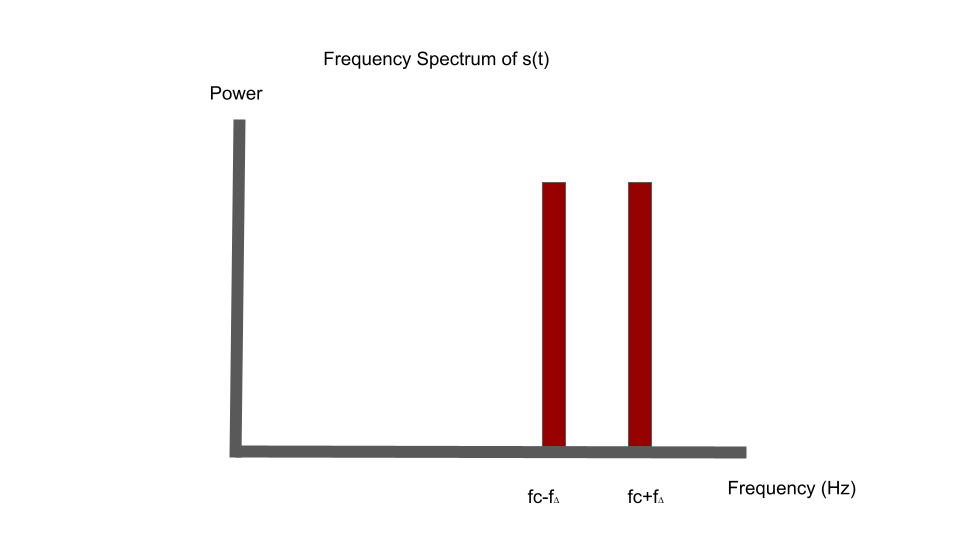
\includegraphics[width=\textwidth]{images/2a.png}
\caption{Frequency distribution of $s(t)$}
\label{fig:2a}
\end{figure}

{\noindent\bf Question 2b.} See the graph in figure \ref{fig:2bi}. However, because of the time scale requested, if plotted with a reasonable amount of plots the graph is just a completely solid colour since the frequencies are so high compared to the time scale. Interestingly, if you accidentally plotted it with an insufficient amount of points (e.g. 200) you would get an aliased signal that looks reasonable except visually looks like a far lower frequency signal. 

When plotted on a more reasonable time scale ($0\leq t\leq 0.1$), the graph looks like figure \ref{fig:2bii}. 

\begin{figure}[htbp]
\centering
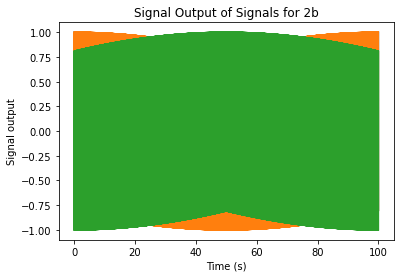
\includegraphics[width=\textwidth]{images/2bi}
\caption{Graph for question 2b. The graph is solid because the frequencies are so high compared to the time scale. }
\label{fig:2bi}
\end{figure}

\begin{figure}[htbp]
\centering
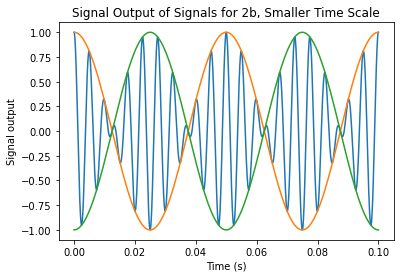
\includegraphics[width=\textwidth]{images/2bii}
\caption{Same graph as in figure \ref{fig:2bi} except on a more reasonable time scale to show actual effects. }
\label{fig:2bii}
\end{figure}

{\noindent\bf Question 2c.} They are called envelopes because the define a window in which $s(t)$, which is more complicated, is always contained under. This can be seen in figure \ref{fig:2bii} which clearly shows the signal $s(t)$ being contained within the given envelopes. 

{\noindent\bf Question 2d.} The pure cosine signal sounds like a low pitch, but $s(t)$ sounds like a pure cosine signal mixed with a higher pitched noise. 

{\noindent\bf Question 2e.} You can see the graph in figure \ref{fig:2e}. 

\begin{figure}[htbp]
\centering
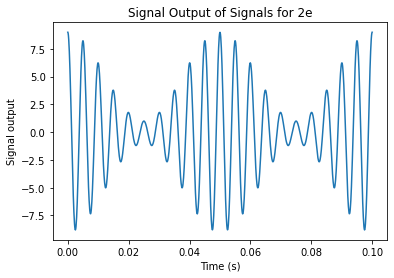
\includegraphics[width=\textwidth]{2e}
\caption{Graph of $s(t)$ for $0\leq t\leq 0.1$}
\label{fig:2e}
\end{figure}

{\noindent\bf Question 2f.} The statement is true. You can see this in figure \ref{fig:2e}, where the carrier wave is clearly visible but it's amplitude varies with the lower frequency signal 

{\noindent\bf Question 2g.} Expanding out the expression, we get 

$$
    s(t) = 5\cos(400\pi t) + 4\cos(40\pi t)\cos(400\pi t)
$$

The second expression is the same as the on in the first part of the question which we know how to decompose, so the three frequency components are 180, 200 and 220Hz. Thus the sketch looks like figure \ref{fig:2g}. 

\begin{figure}[htbp]
\centering
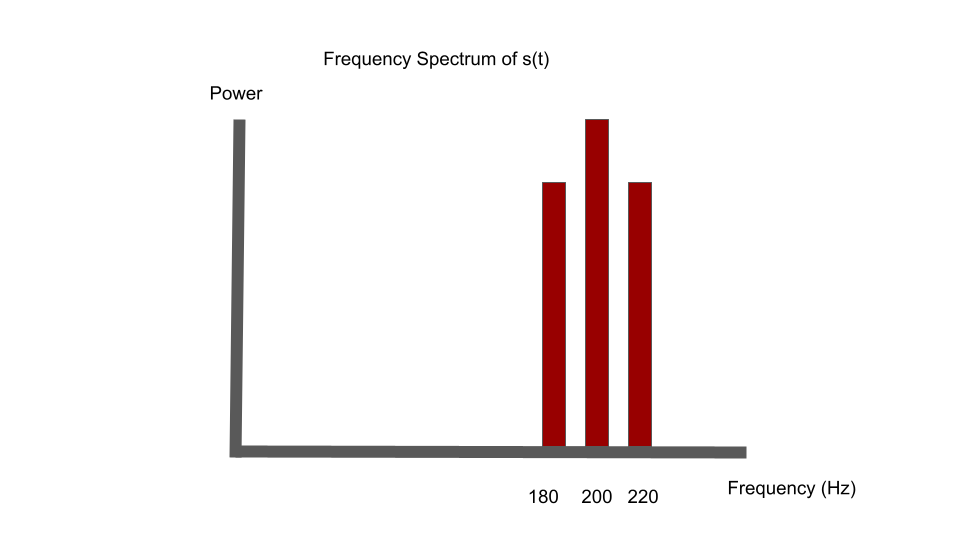
\includegraphics[width=\textwidth]{2g}
\caption{Frequency distribution for question 2g. }
\label{fig:2g}
\end{figure}

{\noindent\bf Question 2h.} The plot can be seen in figure \ref{fig:2h}. The result is obviously quite different from figure \ref{fig:2g} since it is a much lower frequency. Even though visually in the equation the signal from 2g has a lower frequency component, when actually decomposed it only has higher frequency terms. 


\begin{figure}[htbp]
\centering
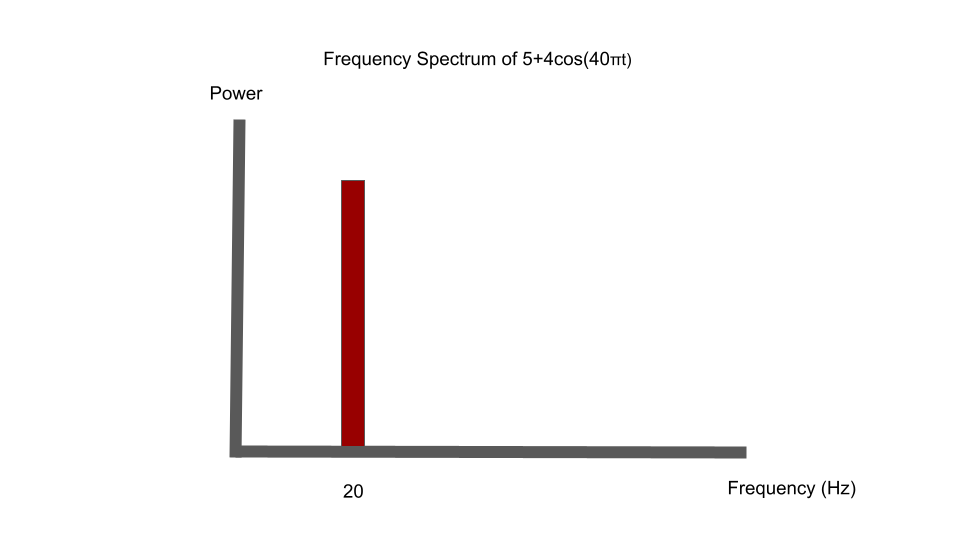
\includegraphics[width=\textwidth]{2h}
\caption{Frequency distribution for question 2h. }
\label{fig:2h}
\end{figure}

{\noindent\bf Question 2i.} The expression would be of the form 

$$
    s(t)=v(t)\cos(2580000\pi t)
$$

$v(t)$ represents the signal being sent, while the argument inside the cosine shows that it is broadcasting at 1290kHz. 

{\noindent\bf Question 2j.} Both $s_1$ and $s_1$ are both in the same form as seen in part e. We already saw in previous parts that for such a signal, when it is decomposed into its frequency components (e.g. during a fourier transform), $s_1$ is purely composed of frequencies of $f_c$, $f_c-f_1$ and $f_c+f_1$ and analogously for $s_2$. For the specific circumstance at hand, this means that when you decompose $r(t)$ into its component frequencies, the frequency between 190 and 200Hz will represent $200-f_1$ and the frequency between 210 and 220 will represent $210+f_2$. 

There is a requirement for $f_1+f_2<10$ because otherwise $f_1$ and $f_2$ run into each when you decompose the signal into its frequencies. By keeping them separate they are clear differentiated and it is possible to recover the original signal. 

{\noindent\bf Question 4.} To find the coefficients for the given function, we use the formula for them: 

$$
    A_0=\frac2T\int_0^{2}x(t)dt={0.5+1}=\frac32
$$
$$
    A_k=\frac2T\int_0^{2}x(t)\cos(\pi kt)dt=\int_0^{0.5}\cos(\pi kt)dt+\int_{1.5}^{2}2\cos(\pi kt)dt
$$
$$
    =\frac{1}{\pi k}(\sin(\pi kt)\bigg|_0^{0.5}+2\sin(\pi kt)\bigg|_{1.5}^2)=\frac{1}{\pi k}(\sin(\frac\pi2k)-2\sin(\frac32\pi k))=\frac{3}{\pi k}\sin(\frac\pi2k)
$$
$$
    B_k=\frac2T\int_0^2f(t)\sin(\pi kt)dt=\int_0^{0.5}\sin(\pi kt)dt+\int_{1.5}^22\sin(\pi kt)dt
$$
$$
    =\frac{1}{\pi k}(-\cos(\pi kt)\bigg|_0^{0.5}-2\cos(\pi kt)\bigg|_{1.5}^2)=\frac1{\pi k}(1-\cos(\frac\pi2k)-2+2\cos(\frac32\pi k))
$$
$$
    =\frac{1}{\pi k}(-1-\cos(\frac\pi2k)+2\cos(\frac32\pi k))=\frac1{\pi k}(\cos(\frac\pi2 k)-1)
$$



\end{document}


